\iffalse
\chapter{Proiectarea aplicației}
\label{cap:cap2}

(10–20 pagini)

\begin{itemize}
    \item se analizează platforma hardware pe care va fi executată respectiva aplicație și se analizează care abordare în implementare ar fi mai bună pentru respectiva structură
    \item se stabilesc modulele generale ale aplicației și interacțiunile dintre ele;
    \item se analizează avantaje și dezavantajele metodei alese;
    \item se indică limitele în care metoda va funcționa. 
\end{itemize}

\textit{Componente software:}
\begin{itemize}
    \item proiectarea propriu zisă (diagrame ER pentru baze de date, UML pentru proiectele care necesită diverse paradigme complexe și lucru cu clase – orientat obiect, scheme logice pentru cei care dezvoltă în limbaje structurate etc);
    \item se stabilește tehnologia aleasă pentru implementare și se justifică alegerea făcută;
    \item se descriu succint numai clasele dezvoltate și implementate de absolvent cu trimitere la pagina din anexă unde se află codul complet;
\end{itemize}

Figurile mai complexe, care nu se văd bine în format A4/portrait, pot fi incluse în anexe și referite normal (vezi Figura \ref{fig:AT} din Anexa \ref{anexa3:func_xyz}).

\vspace{1em}

\textit{Componente hardware:}
\begin{itemize}
    \item stabilirea componentelor hardware necesare. Exemplu: etaje analogice, display-uri, dispozitive I/O, periferice USB, etc.;
    \item analiza performanțelor și descrierea perifericelor procesorului/microcontrolerului folosit
    \item realizarea schemei bloc care să reflecte interconectarea componentelor principale;
    \item simularea funcționării componentelor hardware (OrCAD, Proteus, simulatoare HDL);
    \item proiectarea cablajului imprimat (Altium Designer, Eagle).
\end{itemize}

\textcolor{gray}{\lipsum} (Figura \ref{fig:BB8})

\begin{figure}[H]
    \centering
    
\includegraphics[width=0.3\textwidth]{continut/capitol2/figuri/BB8.png}
    \caption{BB8\protect\footnotemark}
    \label{fig:BB8}
\end{figure}
\footnotetext{imagine preluată de pe un site web care nu „merită” trecut la bibliografie \url{https://www.pngitem.com/}}

\textcolor{gray}{\lipsum}

Ecuația \eqref{eq:sample} este un exemplu foarte simplu de formulă matematică. Ecuațiile vor fi referite prin comanda \LaTeX\ \verb|\eqref{}| din pachetul \verb|amsmath|.

\begin{equation}
    \label{eq:sample}
    e^{\pi i} + 1 = 0
\end{equation}

\begin{equation}
    \label{eq:multiline_sample}
    \begin{split}
        A & = \frac{\pi r^2}{2} \\
         & = \frac{1}{2} \pi r^2
    \end{split}
\end{equation}

În ecuația \eqref{eq:multiline_sample} avem un prim exemplu multiline.

Ecuațiile, definițiile și teoremele se referă în textul lucrării de licență/disertație prefixate: ecuația \eqref{eq:sample}, definiția \ref{def:diploma} sau teorema \ref{thm:equal}, iar aici este o pură întâmplare că au același indice, fiind vorba despre prima ecuație, prima definiție și prima teoremă din Capitolul \ref{cap:cap2}.

În continuare, definiția \ref{def:diploma} introduce conceptul de „Lucrare de diplomă”. Titlul efectiv este opțional și îl regăsiți în \LaTeX\ între [].

\begin{definition}[Lucrare de diplomă]
    \label{def:diploma}
    Lucrarea de diplomă face dovada nivelului și calității pregătirii profesionale, teoretice și aplicative a absolventului, iar prin modul în care aceasta este prezentată (susținută public în fața unei comisii de examinare) ea evidențiază calitățile științifice și inginerești definitorii ale absolventului.
\end{definition}

Numerotarea teoremelor se va face similar ecuațiilor și definițiilor de mai sus. Vezi teorema \ref{thm:equal}.

\begin{theorem}[Teorema egalității]
    \label{thm:equal}
    Dacă $a=b$, atunci $b=a$.
\end{theorem}

\begin{proof}
Ne bazăm pe proprietatea de reflexivitate.
\end{proof}

\textcolor{gray}{\lipsum}

În acest capitol ar trebui să se regăsească un algoritm (dacă este cazul) și el va fi referit ca Algoritmul \ref{alg:acceptance}.

\begin{algorithm}[ht]
    \caption{Pseudo code for reviewing process}\label{alg:acceptance}
    \begin{algorithmic}[1]
        \Procedure{Acceptance}{paper, committee}
            \State $\textit{reviewers} \gets \text{randomly select } \{(i,j) \mid i,j \in  \{1, \cdots, \#\{\textit{committee}\}\}, i \neq j \}$
            \State $\textit{reviews} \gets 2 \times 1 \text{ array of } \textit{False}$
            \BState \emph{reviewing round}:
            \For {$i \in \textit{reviewers }$}
                \If {$paper \text{ reads well for } \textit{committee}(i) $}
                    \State $\textit{review}(i) \gets \textit{True}$.
                \Else \text{ do nothing}
                \EndIf
            \EndFor
            \BState \emph{evaluation round}:
            \If {$\textit{reviews}(i) \text{ is } \textit{False} \text{ for all } i \in \textit{reviewers}$}
                \State \textbf{goto} \emph{hell}.
            \ElsIf {$\textit{reviews}(i) \text{ is } \textit{True} \text{ for all } i \in \textit{reviewers}$}
                \State \textbf{goto} \emph{Licența 2022}
            \Else \textbf{ goto} \emph{revision round}
            \EndIf
            \BState \emph{revision round}:
            \State $\textit{reviser} \gets \text{randomly select } \{i \mid i \in  \{1, \cdots, \#\{\textit{committee}\}\}, i \not\in \textit{reviewers} \}$
            \If {$paper \text{ reads well for } \textit{committee(reviser)} $}
                \State \textbf{ goto} \emph{Licența 2022}
            \ElsIf{\textit{committee(reviser)} \text{ has no opinion and likes inifinite loop}}
                \State \textbf{ goto} \emph{reviewing round}
            \Else \textbf{ goto} \emph{hell}
            \EndIf
            \BState \emph{hell} 
            \State \text{Try again in summer 2023!}
            \BState \emph{Licența 2022 (some people also call it hell)}:
            \State \text{See you at Beer Zone!}
        \EndProcedure
    \end{algorithmic}
\end{algorithm}

\textcolor{gray}{\lipsum}
\fi


\chapter{Proiectarea aplicației}
\label{cap:cap2}

\section{Componente hardware}

\subsection{Calculatorul clasic}

Cum această lucrare se bazează în mare parte și pe măsurarea performanțelor unor algoritmi și metode de generare de numere aleatorii, acest lucru implică și necesitatea de a menționa componentele calculatorului clasic de pe care se vor executa algoritmii. Acolo unde algoritmii și metodele cuantice vor fi simulate strict folosind un calculator clasic, acest lucru va fi menționat explicit. Atunci când voi executa metodele pe un calculator cuantic, voi menționa lucrul acesta. Totuși, în cazul măsurării performanțelor pentru câțiva algoritmi clasici de generare de numere aleatorii, pentru obținerea unui baseline pentru benchmark, se poate presupune că am utilizat un calculator cu următoarele specificații:

\vspace{0.5cm}
\textbf{Laptop I} - Lenovo - Y520
\begin{itemize}
    \item Laptop cu sistemul de operare Windows
    \item 8 GB RAM
    \item CPU Intel i7-7700HQ @ 2.8 GHz, 8 cores
    \item GPU NVidia GeForce GTX 1060 8 GB VRAM, 4 Shared RAM
    \item HDD 1 TB
\end{itemize}

Toate aceste elemente hardware ar putea avea un efect asupra rezultatelor măsurătorilor de performanță în cazul metodelor simulate, dar ideea lucrări este de a compara metodele între ele - nu contează foarte mult valorile propriu-zise rezultate din măsurători!

Totuși, pentru unele metode, cum ar fi citirea din \textit{device}-ul linux \textit{/dev/urandom}, acest lucru va fi, din nou, menționat explicit unde este cazul, iar acest lucru se va face pe un calculator cu următoarele specificații:


\vspace{0.5cm}
\textbf{Laptop II}  - Myria - MY8312SV
\begin{itemize}
    \item Laptop cu sistemul de operare Linux - Xubuntu
    \item 4 GB RAM
    \item CPU Intel Pentium N4200 @ 2.5 GHz, 4 cores
    \item GPU Intel HD Graphics 505
    \item SSD 256 GB
\end{itemize}

În afară de efectul componentelor hardware clasice asupra valorilor absolute de performanță, nu prea există vreo altă componentă hardware care să fie relevantă pentru ansamblul lucrării mele. Am menționat aceste lucruri aici doar pentru a se știe cu ce componente am obținut rezultatele prezentate.

\pagebreak

\subsection{Calculatorul cuantic}
Pentru a menține rigurozitate în măsurătorile de performanță care urmează a fi prezentate, voi folosi pe tot parcursul lucrării un singur calculator cuantic adevărat (prin contrast cu unul simulat), și anume calculatorul IBMQ\_Bogota oferit prin serviciul IBM Quantum Experience. La fel ca și pentru calculatorul clasic, voi lista specificațiile acestui calculator, deoarece toate pot fi importante pentru indicii de performanță obținuți.

Specificațiile calculatorului cuantic sunt următoarele:
\begin{itemize}
    \item 5 Qubiți
    \item 32 Volum Cuantic
    \item 2.3K CLOPS
    \item Tip de procesor: Falcon r4L
    \item Version: 1.6.37
    \item Basis gates: CX, ID, RZ, SX, X
\end{itemize}

Explicațiile specificațiilor sunt următoarele:
\begin{itemize}
    \item Qubiți - Cantitatea de qubiți pe care o are disponibilă calculatorul cuantic; aceștia au o anumită configurație prezentă în figura \ref{fig:TopologieBogota}. Qubiții legați unii de ceilalți pot fi entangled sau se pot executa porți logice cuantice pe mai mulți qubiți între ei, fără a putea face acest lucru între qubiți care nu au conexiune între ei. Conexiunea este fizică și legată strict de design-ul calculatorului cuantic.
    \item Volum Cuantic - O unitate de măsură care reprezintă "dimensiunea" maximă a unui circuit cuantic care poate fi executat de un calculator cuantic. De exemplu, dacă un calculator cuantic cu 8 qubiți poate executa un circuit în care se vor afla maxim 8 stări $\ket{\psi}$ intermediare, atunci spunem că acel calculator are un Volum Cuantic de 256. Prin urmare, volumul cuantic este o specificație de performanță independentă de hardware-ul abstractizat.
    \item CLOPS - Circuit Layer Operations Per Second - Câte straturi de volum cuantic pot fi executate de un QPU (Quantum Processing Unit) într-o unitate de timp. Documentația de la IBM \cite{misc:web:DocumentatieIBMQ} recomandă lectura lucrării \cite{misc:paper:QSS:WackAndrewEtAl} pentru a înțelege conceptul mai bine.
    \item Tipul de procesor: Există o mare varietate de QPU-uri dezvoltate, atât de către IBM, cât și de către alte firme. Familia de procesoare \textit{Falcon} cu seria r4 sunt o platformă pentru circuite de medii dimensiuni, iar calculatorul IBMQ\_Bogota este unul disponibil public, gratuit, prin API-ul cloud de la IBM Quantum Experience.
    \item Versiunea: versiunea procesorului în ansamblu.
    \item Basis gates: porțile compatibile cu QPU-ul dat. Orice circuit care folosește alte porți trebuie \textit{transpilat}, adică trebuiesc descompuse toate celelalte porți în aceste porți pentru a putea fi executat. Qiskit, framework-ul pentru calcul cuantic de la IBM, permite transpilarea automată a oricăror circuite în circuite compatibile cu calculatoarele cuantice disponibile public.
\end{itemize}

\begin{figure}[H]
    \centering
    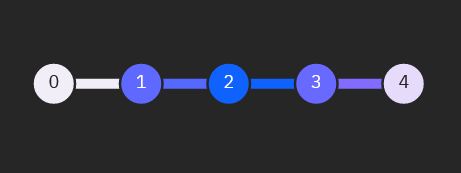
\includegraphics{anexe/figuri/TopologieBogota.png}
    \caption{Topologia fizică a calculatorului cuantic \textit{IBMQ\_Bogota} }
    \label{fig:TopologieBogota}
\end{figure}

\section{Componente software}

\subsection{Limbajul de programare Python}

Limbajul de programare Python este un limbaj de scripting multiparadigmă high-level, interpretat, garbage collected și tipizat dinamic, cu mai multe implementări ale interpretorului în diferite limbaje. Pe parcursul acestei lucrări s-a folosit exclusiv versiunea 3.8 a CPython (Core Python), interpretorul de referință scris în limbajul de programare C. 

Cu apariția necesității unui limbaj de programare pentru calculatoarele cuantice în trecutul recent, mai multe limbaje de programare au fost dezvoltate specific în acest scop, deseori bazate pe limbaje deja existente, cum ar fi limbajul de programare Q\# dezvoltat de Microsoft, care are ca sursă de inspirație limbajul de programare C\#, QCL (Quantum Computation Language), dezvoltat de Institutul pentru Fizică Teoretică, parte a Universității din Viena, una dintre primele limbaje dezvoltate specific pentru programarea calculatoarelor cuantice, cu sintaxă și funcționalitate foarte similară cu cea a limbajului de programare C, QASM sau OpenQASM, limbajul de nivel mijlociu (intermediar) pentru interfațarea cu calculatoarele cuantice de la IBM, limbaj care stă la baza framework-ului ales de mine, și anume Qiskit, dezvoltat în limbajul de programare Python.

Motivul pentru care am ales limbajul Python, împreună cu framework-ul Qiskit, este în mare parte datorită propriei familiarități cu limbajul de programare, fiind una dintre primele limbaje pe care le-am învățat, dar și mulțumită faptului că IBM oferă o gamă destul de largă de calculatoare cuantice pentru interfațare prin API-ul lor. Cum framework-ul dezvoltat specific pentru calculatoarelele lor este Qiskit, framework pentru limbajul Python, interesele s-au aliniat și au contribuit în foarte mare parte la alegerea mea a limbajului. 
Pe lângă aceste lucruri, având în vedere proficiența mea în limbajul de programare, alegând-ul, îl pot folosi în toate nivelurile aplicațiilor mele, de la definirea și executarea circuitelor cuantice, la prelucrarea rezultatelor și analiza statistică a acestora, dar și la dezvoltarea aplicației cu interfață utilizator din ultima parte a proiectului. 

\subsection{Framework-ul Qiskit}


